\section{Maximum entropy state}

\begin{frame}{Quantum maximum entropy principle}
    \begin{columns}
        \begin{column}{0.5\textwidth}
            \begin{itemize}
                \item \textbf{Scenario}: no tomographically complete set of obsevables.
                \item Instead we know $\expval{\hat{G}_{i}}$
            \end{itemize}
            \begin{equation*}
                \Longrightarrow \rho\text{?}
            \end{equation*}
            \vspace{0.1cm}

            \textbf{Maximum Entropy Principle}
            \begin{tcolorbox}
                The density operator that maximizes the entropy is the best estimate of the system's state given some prior data
            \end{tcolorbox}
            \vspace{0.5cm}
        \end{column}
        \begin{column}{0.5\textwidth}
            The von Neumann entropy:
            \begin{equation*}
                S(\rho)=-\Tr(\rho\ln{\rho}).
            \end{equation*}
            Using Lagrange multipliers, the state that maximizes it:
            \begin{equation*}
                \rho_{max}=\frac{1}{Z}e^{\sum_{i}\lambda_{i}\hat{G}_{i}},
            \end{equation*}
            Call it \textbf{maximum entropy state}.
        \end{column}
    \end{columns}
\end{frame}

\begin{frame}{Equivalence between observables}
    \begin{columns}
        \begin{column}{0.5\textwidth}
            Our CG map:
            \begin{equation*}
                \CG{\varrho}=\Tr_{2}((1-p)\varrho+pS\varrho S^{\dag})
            \end{equation*}
            Observables in $\densityspace{2}$ but MaxEnt state in $\densityspace{4}$? No problem!
            \begin{align*}
                \langle \sigma_{i}\rangle=&\Tr{\sigma_{i} \rho}\\
                =&\Tr{\sigma_{i}\otimes\Id((1-p)\varrho+pS\varrho S)}\\
                =&\langle \hat{G}_{i}\rangle.
            \end{align*}
        \end{column}
        \begin{column}{0.5\textwidth}
            Construct $\varrho_{max}$ via
            \begin{equation*}
                \hat{G}_{i}=(1-p)\sigma_{i}\otimes\Id+p\Id\otimes\sigma_{i}.
            \end{equation*}
            as
            \begin{equation*}
                \varrho_{max}=\frac{e^{\lambda (1-p)(\hat{r}_{\rho}\cdot\vec{\sigma})}}{Z_{A}} \otimes \frac{e^{\lambda p(\hat{r}_{\rho}\cdot\vec{\sigma})}}{Z_{B}}.
            \end{equation*}
            Where:
            \begin{itemize}
                \item $\hat{r}_{\rho}$ is $\rho$'s unit Bloch vector
                \item $\lambda=\sqrt{\lambda^{2}_{1}+\lambda^{2}_{2}+\lambda^{2}_{3}}$
            \end{itemize}
        \end{column}
    \end{columns}
\end{frame}

\begin{frame}{Separable MaxEnt}
    \begin{columns}
        \begin{column}{0.5\textwidth}
            MaxEnt state is separable:
            \begin{equation*}
                \varrho_{max}=\rho_{A}\otimes\rho_{B}
            \end{equation*}
            The effective state:
            \begin{equation*}
                \rho=(1-p)\rho_{A}+p\rho_{B}
            \end{equation*}
        \end{column}
        \begin{column}{0.5\textwidth}
            \begin{figure}[h!]
                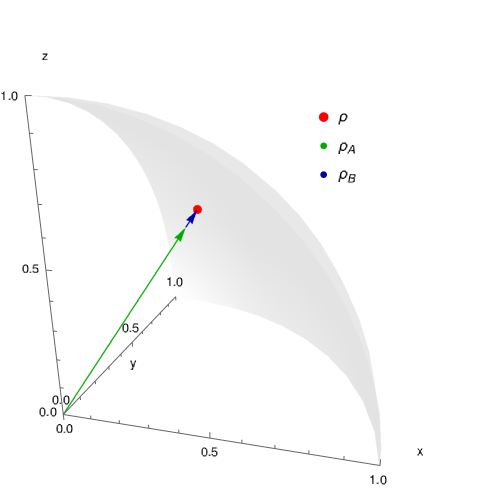
\includegraphics[width=0.75\columnwidth]{figures/effective_state_as_sum.png}%
                \caption{Effective state decomposed. $p=0.2$}
            \end{figure}
        \end{column}
    \end{columns}
\end{frame}

\begin{frame}{Quick review}
    \begin{displaymath}
        \xymatrix{
          {\rho(0)} \ar[rr]^{\Gamma_{t}} \ar[d]^{\mcA^{max}_{\mcC}}
          && {\rho(t)}\\
          {\varrho_{max}(0)} \ar[rr]^{\mcU_{t}}
          && {\varrho_{max}(t)} \ar[u]^{\mcC}
        }
      \end{displaymath}
      Where:
        \begin{equation*}
            \mcA_{\mcC}^{\max}[\rho]=\varrho_{max}=\rho_{A}\otimes\rho_{B} \qquad \mcU_{t}[\rho]=U^{t}\varrho(U^{t})^{\dag} \qquad \CG{\varrho}=\Tr_{2}((1-p)\varrho+pS\varrho S^{\dag})
        \end{equation*}
        \begin{equation*}
            \boxed{\Gamma_t[\rho]:=(\mcC \circ \mcU_t \circ \mcA^{max}_{\mcC})[\rho].}
        \end{equation*}
\end{frame}